\documentclass[12pt, titlepage]{article}

\usepackage{fullpage}
\usepackage[round]{natbib}
\usepackage{multirow}
\usepackage{booktabs}
\usepackage{tabularx}
\usepackage{graphicx}
\usepackage{float}
\usepackage{hyperref}
\hypersetup{
    colorlinks,
    citecolor=black,
    filecolor=black,
    linkcolor=red,
    urlcolor=blue
}
\usepackage[round]{natbib}
\usepackage{xifthen}

\newcounter{acnum}
\newcommand{\actheacnum}{AC\theacnum}
\newcommand{\acref}[1]{AC\ref{#1}}

\newcounter{ucnum}
\newcommand{\uctheucnum}{UC\theucnum}
\newcommand{\uref}[1]{UC\ref{#1}}

\newcounter{mnum}
\newcommand{\mthemnum}{M\themnum}
\newcommand{\mref}[1]{M\ref{#1}}
\newcommand{\newterm}[1]{\label{Term:#1} \MakeUppercase #1}
\newcommand{\term}[2][]{\ifthenelse{\equal{#1}{}}{\hyperref[Term:#2]{\textbf{#2}}}{\hyperref[Term:#1]{\textbf{#2}}}}

\title{SE 3XA3: Software Requirements Specification\\Random Flag Generator}

\author{Team \#2, Team Jakriel
		\\ Akram Hannoufa, hannoufa
		\\ Ganghoon (James) Park, parkg10
		\\ Nathaniel Hu, hun4
}

\date{\today}

% \input{../../Comments}

\begin{document}

\maketitle

\pagenumbering{roman}
\tableofcontents
\listoftables
\listoffigures

\begin{table}[bp]
\caption{\bf Revision History}
\begin{tabularx}{\textwidth}{p{3cm}p{2cm}X}
\toprule {\bf Date} & {\bf Version} & {\bf Notes}\\
\midrule
March 15, 2022 & 1.0 & Initial Document\\
March 16, 2022 & 1.1 & Added initial drafts of Module Hierarchy and Module Decomposition Sections\\
March 17, 2022 & 1.2 & Added initial draft of Anticipated and Unlikely Changes Section; added uses hierarchy diagram to Use Hierarchy Between Modules Section; added traceability matrices to Traceability Matrix Section\\
March 17, 2022 & 1.3 & Added and modified Intro and Connection sections.\\
\bottomrule
\end{tabularx}
\end{table}

\newpage

\pagenumbering{arabic}

\section{Introduction}
Flag Generator is an implementation of the open-source project PAGAN,
Python Avatar Generation for Absolute Nerds. The main functionality of the program
comes from generating a hashcode from a user's input string and creating a unique
graphical output based on the generated hashcode. Flag Generator generates a unique flag
with its own set of colours, symbols, designs, etc. all based on the hashcode generated from
the user's input.
\subsection{Purpose}
The purpose of the Module Guide document is to outline how this system is modularly 
decomposed. Following a module decomposition approach, the information hiding 
principle is being adhered to~\citep{Parnas1972a}. Following this principle also allows
new project members, maintainers, and designers to be able to easily identify the 
individual components of the software, derive an understanding of the hierarchical structure
of the system, and to easily verify certain software criteria such as consistency, flexibility,
 and feasibility. Additionally, by breaking up the system into modules, the principles
 of low cohesion and high coupling.

\subsection{Scope}
The modules used to develop this program were based off of the requirements outlined in 
the Software Requirements Specification. The modules' external behaviours are 
explicitly described and outlined in the corresponding Module Interface Specification document.
Through adhering to the principle of information hiding, anticipated and unlikely changes 
are represented by the secrets of the modules, allowing for easier changes to be made in the future 
(design for change). Lastly, a uses hierarchy is established to grpahically show
the relationships between the modules.
\newpage
\subsection{Acronyms, Abbreviations, and Symbols}
    
\begin{table}[htbp]
\caption{\textbf{Table of Abbreviations}} \label{abbrev}

\begin{tabularx}{\textwidth}{p{3cm}X}
\toprule
\textbf{Abbreviation} & \textbf{Definition} \\
\midrule
\newterm{GUI} & Graphical User Interface\\
\hline
\newterm{UI} & User Interface\\
\hline
\newterm{FR} & Functional Requirement\\
\hline
\newterm{RGB} & Red Green Blue\\
\hline
\newterm{SRS} & Software Requirements Specification\\
\hline
\newterm{PAGAN} & \term{Python Avatar Generator for Absolute Nerds}\\
\bottomrule
\end{tabularx}

\end{table}

\newpage
\begin{table}[htbp]
\caption{\textbf{Table of Definitions}} \label{def}

\begin{tabularx}{\textwidth}{p{3cm}X}
\toprule
\textbf{Term} & \textbf{Definition}\\
\midrule
    \newterm{Python} & The programming language used in this project.\\
    \hline
    \newterm{Pytest} & Python testing tool that allows testers to write test
    code and create simple and scalable test cases.\\
    \hline
    \newterm{Input String} & The input of type string from the user.\\
    \hline
    \newterm{Gallery} & Collection of previously generated flags.\\
    \hline
    \newterm{Hashing} & Algorithm that converts input data to a fixed-size
    value. A hashing function usually outputs a string or hexadecimal value.\\
    \hline
    \newterm{User} & Person who uses or operates a computer program.\\
    \hline
    \newterm{User Interface} & Where interactions between machines and humans
    occur.\\
    \hline
    \newterm{Graphical User Interface} & A form of UI that allows users to use
    electronic devices using interactive graphics.\\
    \hline
    \newterm{System/Program} & Collection of instructions or components that
    tell a computer how to operate.\\
    \hline
    \newterm{Software Requirements Specification} & A document that details
    what the program/software will do and how it will accomplish the expected
    performance/tasks.\\
    \hline
    \newterm{Tester} & An individual testing the software via the user
    interface or the code/test cases.\\
    \hline
    \newterm{Typeform} & Website that is a software as a service that
    specializes in creating and building online surveys.\\

\bottomrule
\end{tabularx}
    
\end{table} 

\newpage
\subsection{Overview}
The rest of the document is organized as follows. 
\begin{itemize}
  \item Section \ref{SecChange}: Lists the anticipated and unlikely changes of the software
  requirements.
  \item Section \ref{SecMH}: Summarizes the module decomposition that
  was constructed according to the likely changes.
  \item Section \ref{SecConnection}: Specifies the connections between the software requirements and the modules.
  \item Section \ref{SecMD}: Gives a detailed description of the
  modules.
  \item Section \ref{SecTM}: Includes two traceability matrices. One checks
  the completeness of the design against the requirements provided in the SRS. The
  other shows the relation between anticipated changes and the modules.
  \item Section \ref{SecUse}: Describes the use relation between modules.
\end{itemize}
\section{Anticipated and Unlikely Changes} \label{SecChange}

This section lists possible changes to the system. According to the likeliness
of the change, the possible changes are classified into two
categories. Anticipated changes are listed in Section \ref{SecAchange}, and
unlikely changes are listed in Section \ref{SecUchange}.

\subsection{Anticipated Changes} \label{SecAchange}

Anticipated changes are the source of the information that is to be hidden
inside the modules. Ideally, changing one of the anticipated changes will only
require changing the one module that hides the associated decision. The approach
adapted here is called design for
change.

\begin{description}
\item[\refstepcounter{acnum} \actheacnum \label{ac1}:] The addition of new flag assets.
\item[\refstepcounter{acnum} \actheacnum \label{ac2}:] The flag resolution options.
\item[\refstepcounter{acnum} \actheacnum \label{ac3}:] Available hashing functions.
\item[\refstepcounter{acnum} \actheacnum \label{ac4}:] Maximum size of flag gallery (number of images).
\item[\refstepcounter{acnum} \actheacnum \label{ac5}:] Where and how flags are displayed after being generated.
\item[\refstepcounter{acnum} \actheacnum \label{ac6}:] More user control over user input streams; output.
\item[\refstepcounter{acnum} \actheacnum \label{ac7}:] Output file format.
\item[\refstepcounter{acnum} \actheacnum \label{ac8}:] Input string criteria, wider range of allowable characters (broader input range).
\item[\refstepcounter{acnum} \actheacnum \label{ac9}:] Making changes to how to use the program.

\end{description}

\subsection{Unlikely Changes} \label{SecUchange}

The module design should be as general as possible. However, a general system is
more complex. Sometimes this complexity is not necessary. Fixing some design
decisions at the system architecture stage can simplify the software design. If
these decision should later need to be changed, then many parts of the design
will potentially need to be modified. Hence, it is not intended that these
decisions will be changed.

\begin{description}
\item[\refstepcounter{ucnum} \uctheucnum \label{uc1}:] The same graphics library (PIL/pillow) will be used to generate the flag image files 
\item[\refstepcounter{ucnum} \uctheucnum \label{uc2}:] The same asset reader (JKAReader) will be used to read the flag symbol design.
\item[\refstepcounter{ucnum} \uctheucnum \label{uc3}:] String input 
\item[\refstepcounter{ucnum} \uctheucnum \label{uc4}:] Input/output devices (input: keyboard, output: monitor and file)
\item[\refstepcounter{ucnum} \uctheucnum \label{uc5}:] Hashing function  
\end{description}

\section{Module Hierarchy} \label{SecMH}

This section provides an overview of the module design. Modules are summarized
in a hierarchy decomposed by secrets in Table \ref{TblMH}. The modules listed
below, which are leaves in the hierarchy tree, are the modules that will
actually be implemented.

\begin{description}
\item [\refstepcounter{mnum} \mthemnum \label{M1}:] HashGenerator Module
\item [\refstepcounter{mnum} \mthemnum \label{M2}:] FlagAssetsLib Module
\item [\refstepcounter{mnum} \mthemnum \label{M3}:] JKAReader Module
\item [\refstepcounter{mnum} \mthemnum \label{M4}:] DecisionUtilities Module
\item [\refstepcounter{mnum} \mthemnum \label{M5}:] HashToFlag Module
\item [\refstepcounter{mnum} \mthemnum \label{M6}:] FlagGenerator Module
\item [\refstepcounter{mnum} \mthemnum \label{M7}:] GUI Module
\item [\refstepcounter{mnum} \mthemnum \label{M8}:] Display Module
\item [\refstepcounter{mnum} \mthemnum \label{M9}:] Gallery Module
\item [\refstepcounter{mnum} \mthemnum \label{M10}:] HelpInstructions Module
\item [\refstepcounter{mnum} \mthemnum \label{M11}:] Settings Module
\end{description}


\begin{table}[h!]
\centering
\begin{tabular}{p{0.3\textwidth} p{0.6\textwidth}}
\toprule
\textbf{Level 1} & \textbf{Level 2}\\
\midrule

{Hardware-Hiding Module} & ~ \\
\midrule

\multirow{7}{0.3\textwidth}{Behaviour-Hiding Module} & HashGenerator \\
& FlagAssetsLib \\
& JKAReader \\
& GUI \\
& Display \\
& Gallery \\ 
& HelpInstructions \\
& Settings \\
\midrule

\multirow{3}{0.3\textwidth}{Software Decision Module} & DecisionUtilities \\
& HashToFlag \\
& FlagGenerator \\
\bottomrule

\end{tabular}
\caption{Module Hierarchy}
\label{TblMH}
\end{table}

\section{Connection Between Requirements and Design} \label{SecConnection}

The design of the system is intended to satisfy the requirements developed in
the SRS. In this stage, the system is decomposed into modules. The connection
between requirements and modules is listed in Table \ref{TblRT}, in the form of a traceability matrix. 

Every functional requirement is implemented by at least one module, and similarly
the modules responsible for handling the anticipated changes are also laid out in a traceability matrix, Table \ref{TblACT}.

Modules are generally broken up into hash generation, hashcode to flag decisions and GUI modules. Within these
categories, there is a breakdown of modules to handle specific functionalities. The GUI functionality is broken down
into Display, Gallery, Help, and Settings modules to handle specific funcional requirements. Similarly, HashToFlag's functionality is broken down
into a FlagAssetsLib, HashGenerator (module responsible for generating the hashcode), and a DecisionUtilities module (helper functions for converting a hashcode to decisions).
Lastly, the JKAReader module (responsible for converting .jka files into pixels) combined with the HashToFlag module comprises the majority of the FlagGenerator functionality.


\section{Module Decomposition} \label{SecMD}

Modules are decomposed according to the principle of ``information hiding''
proposed by \citet{ParnasEtAl1984}. The \emph{Secrets} field in a module
decomposition is a brief statement of the design decision hidden by the
module. The \emph{Services} field specifies \emph{what} the module will do
without documenting \emph{how} to do it. For each module, a suggestion for the
implementing software is given under the \emph{Implemented By} title. If the
entry is \emph{OS}, this means that the module is provided by the operating
system or by standard programming language libraries.  

\subsection{Hardware Hiding Modules}

N/A

% \begin{description}
% \item[Secrets:]The data structure and algorithm used to implement the virtual
%   hardware.
% \item[Services:]Serves as a virtual hardware used by the rest of the
%   system. This module provides the interface between the hardware and the
%   software. So, the system can use it to display outputs or to accept inputs.
% \item[Implemented By:] OS
% \end{description}

\subsection{Behaviour-Hiding Module}

\subsubsection{HashGenerator Module (\mref{M1})}

\begin{description}
\item[Secrets:] Hashing algorithms available and method for generating hash
  digests from input strings and selected hashing algorithm (if available)
\item[Services:] Generates hash digests from input strings using selected
  hashing algorithms (if available; default algorithm is SHA-256)
\item[Implemented By:] Random Flag Generator
\end{description}

\subsubsection{FlagAssetsLib Module (\mref{M2})}

\begin{description}
\item[Secrets:] Flag assets, constants and values used to generate flags
\item[Services:] Provides the data files and values needed to generate flags
\item[Implemented By:] Random Flag Generator
\end{description}

\subsubsection{JKAReader Module (\mref{M3})}

\begin{description}
\item[Secrets:] Method for parsing flag asset (.jka) file data into usable
  form for generating flags
\item[Services:] Parses flag asset (.jka) file data into pixel maps to be used
  to generate flags
\item[Implemented By:] Random Flag Generator
\end{description}

\subsubsection{GUI Module (\mref{M4})}

\begin{description}
\item[Secrets:] Methods for starting the program and presenting the GUI view,
  taking in user input strings and selected settings for generating flags
\item[Services:] Starts the program and presents the GUI view, takes in user
  input strings and selected settings for generating flags
\item[Implemented By:] Random Flag Generator
\end{description}

\subsubsection{Display Module (\mref{M5})}

\begin{description}
\item[Secrets:] Methods for displaying the associated generated flags
\item[Services:] Displays the associated generated flags via a GUI
\item[Implemented By:] Random Flag Generator
\end{description}

\subsubsection{Gallery Module (\mref{M6})}

\begin{description}
\item[Secrets:] Saved flags in user's flag gallery and methods for displaying
  all saved flags from the user's flag gallery and searching up flags by
  name (i.e. input string)
\item[Services:] Displays all the saved flags from the user's flag gallery via
  an interactive GUI
\item[Implemented By:] Random Flag Generator
\end{description}

\subsubsection{HelpInstructions Module (\mref{M7})}

\begin{description}
\item[Secrets:] Help and instructions information and methods for displaying
  the help and instructions menu
\item[Services:] Displays the helps and instructions menu and information via
  a GUI
\item[Implemented By:] Random Flag Generator
\end{description}

\subsubsection{Settings Module (\mref{M8})}

\begin{description}
\item[Secrets:] Program version and methods for displaying the settings menu,
  taking in user settings changes and updating settings
\item[Services:] Displays the settings menu and program version via an
  interactive GUI
\item[Implemented By:] Random Flag Generator
\end{description}

\subsection{Software Decision Module}

\subsubsection{DecisionUtilities Module (\mref{M9})}

\begin{description}
\item[Secrets:] Auxiliary helper methods for padding generated hash digests
  (that are too short) and assisting in flag generation information parsing
  and usage in generating flags, and associated constants and values that will
  be used by the auxiliary helper methods
\item[Services:] Pads generated hash digests (that are too short) and assists
  in flag generation information parsing and usage in generating flags
\item[Implemented By:] Random Flag Generator
\end{description}

\subsubsection{HashToFlag Module (\mref{M10})}

\begin{description}
\item[Secrets:] Methods for grinding generated hash digests to select the
  colours and flag design elements to generate flags
\item[Services:] Provides the selected colours and flag design elements
  obtained from grinding the generated hash digest to generate flags
\item[Implemented By:] Random Flag Generator
\end{description}

\subsubsection{FlagGenerator Module (\mref{M11})}

\begin{description}
\item[Secrets:] Methods for obtaining the colours and flag design elements and
  generating the flags and saving the flag image files to the flag gallery
\item[Services:] Obtains the colours and flag design elements and generates
  the flags and saves the flag image files to the flag gallery
\item[Implemented By:] Random Flag Generator
\end{description}

\section{Traceability Matrix} \label{SecTM}

This section shows two traceability matrices: between the modules and the
requirements and between the modules and the anticipated changes.

% the table should use mref, the requirements should be named, use something
% like fref
\begin{table}[H]
\centering
\begin{tabular}{p{0.2\textwidth} p{0.6\textwidth}}
\toprule
\textbf{Req.} & \textbf{Modules}\\
\midrule
FR1 & \mref{M7}\\
FR2 & \mref{M7}\\
FR3 & \mref{M7}\\
FR4 & \mref{M1}, \mref{M2}, \mref{M3}, \mref{M4}, \mref{M5}, \mref{M6}, \mref{M7}\\
FR5 & \mref{M8}\\
FR6 & \mref{M1}, \mref{M2}, \mref{M3}, \mref{M4}, \mref{M5}, \mref{M6}, \mref{M11}\\
FR7 & \mref{M6}\\
FR8 & \mref{M1}, \mref{M2}, \mref{M3}, \mref{M4}, \mref{M5}, \mref{M6}, \mref{M7}\\
FR9 & \mref{M8}\\
FR10 & \mref{M1}, \mref{M2}, \mref{M3}, \mref{M4}, \mref{M5}, \mref{M6}, \mref{M11}\\
FR11 & \mref{M6}, \mref{M7}, \mref{M9}\\
FR12 & \mref{M10}\\
FR13 & \mref{M10}\\
FR14 & \mref{M11}\\
FR15 & \mref{M11}\\
FR16 & \mref{M11}\\
FR17 & \mref{M9}\\
FR18 & \mref{M9}\\
FR19 & \mref{M9}\\
\bottomrule
\end{tabular}
\caption{Trace Between Requirements and Modules}
\label{TblRT}
\end{table}

\begin{table}[H]
\centering
\begin{tabular}{p{0.2\textwidth} p{0.6\textwidth}}
\toprule
\textbf{AC} & \textbf{Modules}\\
\midrule
\acref{ac1} & \mref{M2}, \mref{M3}\\
\acref{ac2} & \mref{M2}\\
\acref{ac3} & \mref{M1}\\
\acref{ac4} & \mref{M9}\\
\acref{ac5} & \mref{M8}\\
\acref{ac6} & \mref{M4}, \mref{M5}, \mref{M6}, \mref{M7}, \mref{M11}\\
\acref{ac7} & \mref{M6}\\
\acref{ac8} & \mref{M1}, \mref{M7}\\
\acref{ac9} & \mref{M10}\\
\bottomrule
\end{tabular}
\caption{Trace Between Anticipated Changes and Modules}
\label{TblACT}
\end{table}

\section{Use Hierarchy Between Modules} \label{SecUse}

In this section, the uses hierarchy between modules is
provided. \citet{Parnas1978} said of two programs A and B that A {\em uses} B if
correct execution of B may be necessary for A to complete the task described in
its specification. That is, A {\em uses} B if there exist situations in which
the correct functioning of A depends upon the availability of a correct
implementation of B.  Figure \ref{FigUH} illustrates the use relation between
the modules. It can be seen that the graph is a directed acyclic graph
(DAG). Each level of the hierarchy offers a testable and usable subset of the
system, and modules in the higher level of the hierarchy are essentially simpler
because they use modules from the lower levels.

\begin{figure}[H]
\centering
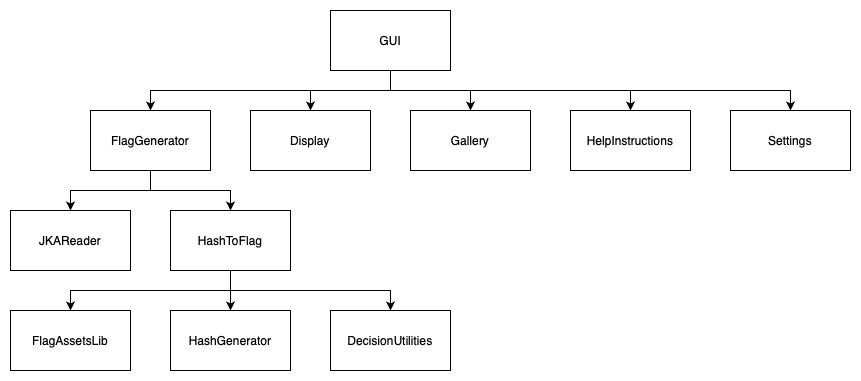
\includegraphics[width=1.0\textwidth]{UsesHierarchy.png}
\caption{Use hierarchy among modules}
\label{FigUH}
\end{figure}


\bibliographystyle {plainnat}
\bibliography {MG}

\end{document}